\begin{figure}[H]
    \centering
    \vfill

    \begin{subfigure}{0.28\textwidth} 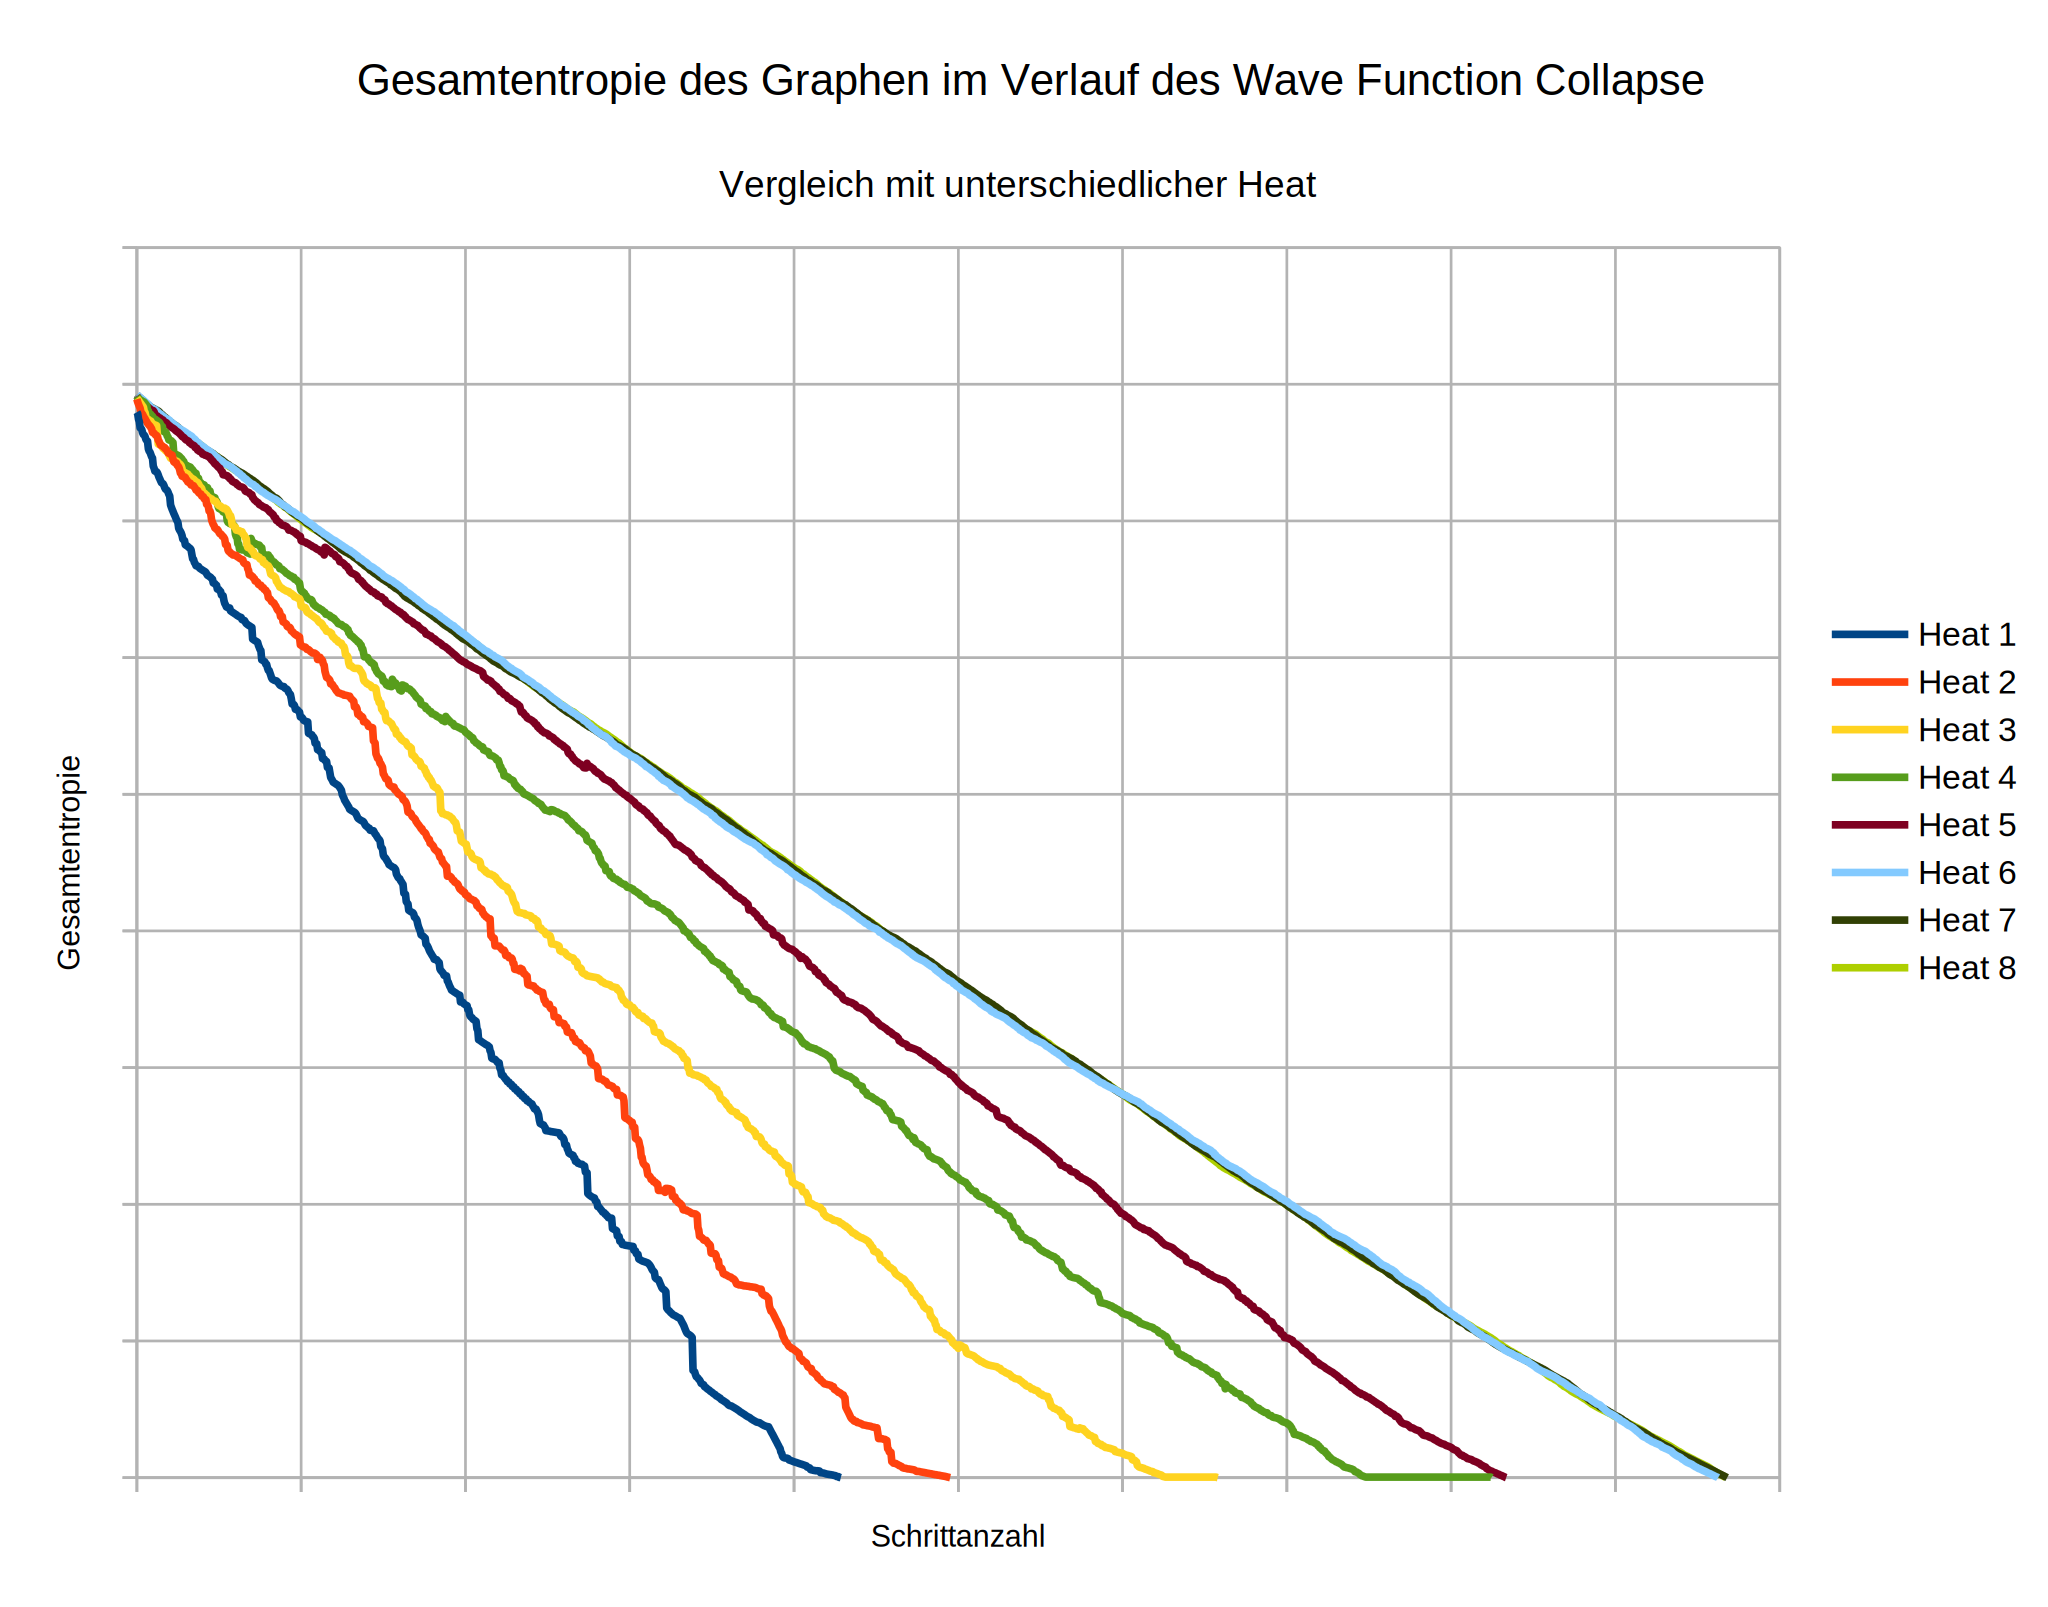
\includegraphics[width=\linewidth]{data/graph_examples/1.png}  \caption{} \end{subfigure}
    \begin{subfigure}{0.28\textwidth} \includegraphics[width=\linewidth]{data/graph_examples/2.png}  \caption{} \end{subfigure}
    \begin{subfigure}{0.28\textwidth} \includegraphics[width=\linewidth]{data/graph_examples/3.png}  \caption{} \end{subfigure}
    \begin{subfigure}{0.28\textwidth} \includegraphics[width=\linewidth]{data/graph_examples/4.png}  \caption{} \end{subfigure}
    \begin{subfigure}{0.28\textwidth} \includegraphics[width=\linewidth]{data/graph_examples/5.png}  \caption{} \end{subfigure}
    \begin{subfigure}{0.28\textwidth} \includegraphics[width=\linewidth]{data/graph_examples/6.png}  \caption{} \end{subfigure}
    \begin{subfigure}{0.28\textwidth} \includegraphics[width=\linewidth]{data/graph_examples/7.png}  \caption{} \end{subfigure}
    \begin{subfigure}{0.28\textwidth} \includegraphics[width=\linewidth]{data/graph_examples/8.png}  \caption{} \end{subfigure}
    \begin{subfigure}{0.28\textwidth} \includegraphics[width=\linewidth]{data/graph_examples/9.png}  \caption{} \end{subfigure}
    \begin{subfigure}{0.28\textwidth} \includegraphics[width=\linewidth]{data/graph_examples/10.png} \caption{} \end{subfigure}
    \begin{subfigure}{0.28\textwidth} \includegraphics[width=\linewidth]{data/graph_examples/11.png} \caption{} \end{subfigure}
    \begin{subfigure}{0.28\textwidth} \includegraphics[width=\linewidth]{data/graph_examples/12.png} \caption{} \end{subfigure}
    
    \caption{
        Beispiele für generierte Graphen. Punkte vom Nutzer(Rot), Delaunay-Triangulierung(Gelb), Voronoi-Diagramm(Grün). 
        Es können regelmäßige gitter-ähnliche (a-c, d-f) oder rein zufällig angeordnete (g-i) Graphen entstehen. In (j-l) sind Teile des Graphen gitterartig während andere zufällige oder kreisförmige Anordnungen haben.
    }
    \label{fig:graph_examples}
    
    \vfill
\end{figure}